%%%%%%%%% BODY TEXT
\section{AutoEncoder-Based Multicut Approach}
\label{subsec:method}
The proposed approach is based on the idea to learn, from simple spatial data associations between object detections in image sequences, which appearance variations are to be expected within one object for the task of multiple object tracking \AK{this sentence is not clear to me}. An overview of our workflow implementing this idea is given in Fig.~\ref{fig:figure0}.

\textbf{Stage 1.} 
The object detection bounding boxes are extracted along with their spatial information such that spatial correspondences between detections in neighboring frames can be computed.
Based on these simple spatial associations, detections can be grouped into tracklets in order to obtain cluster labels using clustering approaches such as correlation clustering, also referred to as minimum cost multicuts~\cite{demaine-2006}.

\textbf{Stage 2.} 
A convolutional AutoEncoder is trained to learn the visual features of detections. 
The objective is to learn a latent space representation which can serve to match the same object in different video frames. 
Thus, the information about spatial cluster labels from the first stage is used as the centroid of latent features. 
Distances between latent representations of data samples and their centroids are minimized in the convolutional AutoEncoder using a clustering loss. 

Lastly, the data are transformed into the latent space of the trained AutoEncoder to extract pairwise appearance distances which are expected to encode the desired invariances. 
Such pairwise appearance distances are used to not only provide additional grouping information between nearby detections, but also for detections with long temporal distance. 
The final detection grouping is computed using minimum cost lifted multicuts~\cite{keupericcv}.

This section is divided into three subsections: 
Section \ref{subsec:multicut} describes the minimum cost (lifted) multicut approach employed for obtaining the initial spatial cluster labels (e.g. tracklets), as well as for the generation of the final tracking result. Section \ref{subsec:autoencoder} describes the feature learning process using a convolutional AutoEncoder and cluster labels, and section~\ref{subsec:affinity} describes the computation of the joint spatial and appearance metrics used in the final data association step within the minimum cost lifted multicut framework.

\begin{figure*}[t]
	\begin{center}
		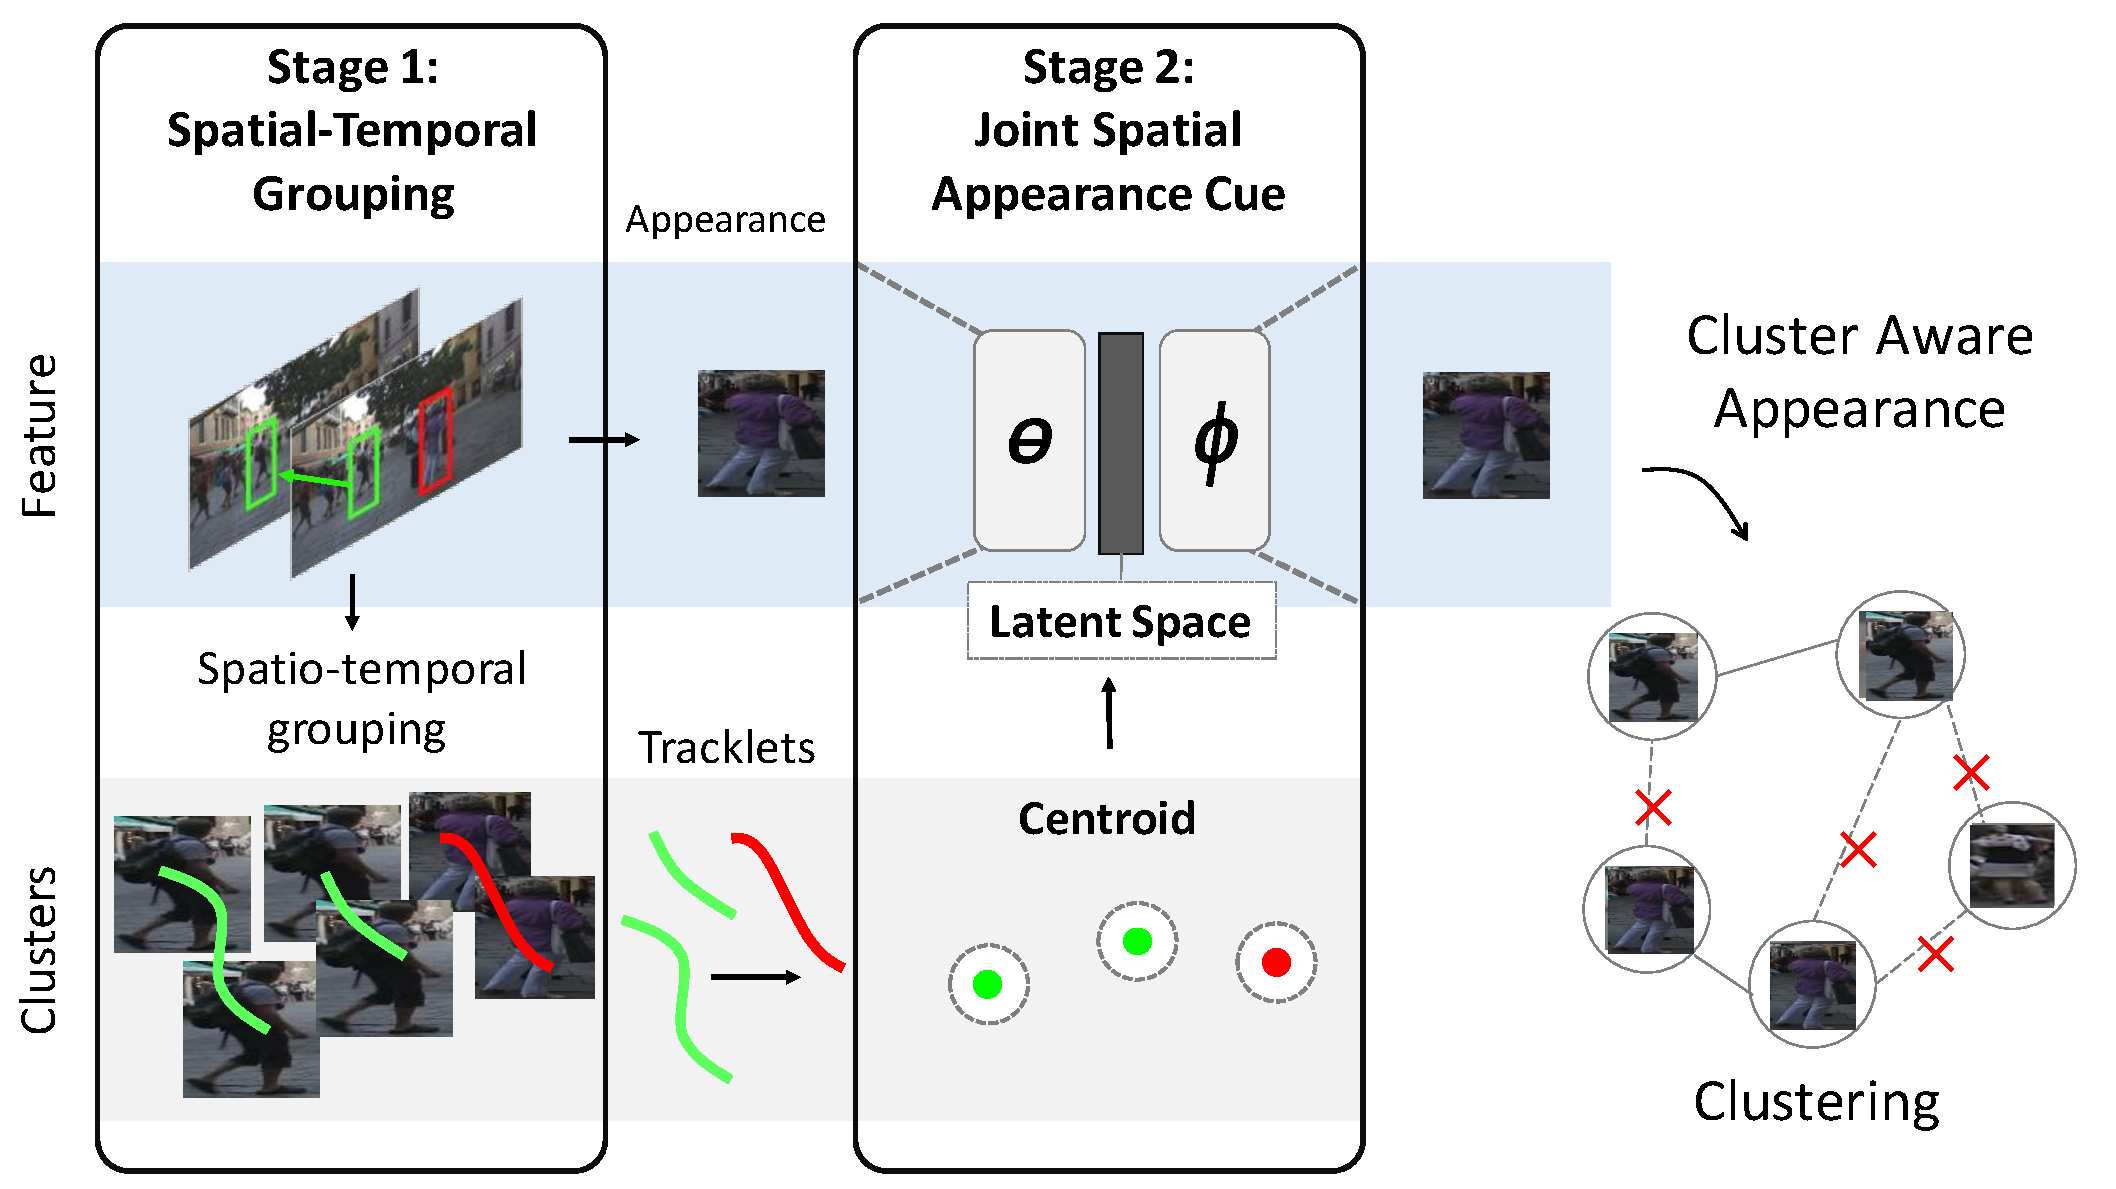
\includegraphics[width=0.9\linewidth]{Fig_2_figure2.pdf}
	\end{center}
	\caption{Summary of our approach in two steps: 1. Initial multicut clustering to obtain weak cluster labels (tracklets), 2. Learn visual features by an AutoEncoder in order to extract affinity information to obtain final clustering (tracking) using lifted multicuts.}
	\label{fig:figure0}
\vspace*{-5mm}
\end{figure*}

\subsection{Multicut Formulation}
\label{subsec:multicut}

We follow Tang~\cite{tang2017multiple} and phrase the multiple target tracking problem as a graph partitioning problem, more concretely, as a minimum cost (lifted) multicut problem. This formulation can serve as well for an initial tracklet generation process, which will help us to inject cues learned from spatial information into the appearance features, as it can be used to generate the final tracking result using short- and long-range information between object detections. \\

\noindent\textbf{Minimum Cost Multicut Problem}.
%%%
We assume, we are given an undirected graph {\it $G = (V, E)$}, where nodes $v\in V$ represent object detections and edges $e\in E$ encode their respective spatio-temporal connectivity. 
Additionally, we are given real valued costs {\it $c: E \rightarrow \mathbb{R}$} defined on all edges. 
Our goal is to determine \emph{edge} labels {\it $y: E \rightarrow \{0, 1\}$} defining a graph decomposition such that every partition of the graph corresponds to exactly one object track (or tracklet). 
To infer such an edge labeling, we can solve instances of the minimum cost multicut problem with respect to the graph G and costs c, defined as follows \cite{chopra-1993,demaine-2006}:

\begin{align}
\min\limits_{y \in \{0, 1\}^E}
\sum\limits_{e \in E} c_e y_e
\label{eq:mc}
\end{align}

\begin{align}
s.t. \quad \forall C \in cycles(G) \quad \forall e \in C : y_e \leq \sum\limits_{e^\prime \in C\backslash\{e\}} y_{e^\prime}
\label{eq:cycle}
\end{align}
Here, the objective is simply to cut those edges with negative costs $c_e$ such that the resulting cut is a decomposition of the graph. 
This condition is formalized by the cycle inequalities in Eq.~\eqref{eq:cycle}, which make sure that, for every cycle in $G$, if one of its edges is cut, so is at least one other.
Thus, no two nodes can remain connected via some path of the graph if an edge is cut between them along any other path. 
In \cite{chopra-1993}, it was shown to be sufficient to enforce Eq.~\eqref{eq:cycle} on all \emph{chordless} cycles, i.e. all cycles.

Typically, if cut probabilities between pairs of nodes are available, the costs are computed using the \emph{logit} function $\text{logit}(p) = \log\frac{p}{1-p}$  to generate positive and negative costs.
With these costs set appropriately, the optimal solution of minimum cost multicut problems not only yields an optimal cluster assignment but also estimates the number of clusters (e.g. objects to track) automatically. 

While the plain minimum cost multicut problem has shown good performance in multiple object tracking scenarios with only short range information available~\cite{tang2016multi}, the cost function actually has a rather limited expressiveness. 
In particular, when we want to add connectivity cues between temporally distant bounding boxes, we can only do so by inserting a direct edge into the graph. 
This facilitates solutions that directly connect such distant nodes even if this link is not justified by any path through space and time. 
This limitation is alleviated by the formulation of minimum cost \emph{lifted} multicuts~\cite{keupericcv}.\\

\noindent\textbf{Minimum Cost Lifted Multicut Problem}.
%%%
For a given, undirected graph $G = (V, E)$ and an additional edge set $F\subseteq \binom{V}{2} \setminus E$ and any  real valued cost function $c: E \cup F \to \mathbb{R}$,
the 01 linear program written below is an instance of the
\emph{Minimum Cost Lifted Multicut Problem (LMP)}
w.r.t.~$G$, $F$ and $c$~\cite{keupericcv}:
%
\begin{equation}
\displaystyle\min_{y \in Y_{EF}} 
    \quad \sum_{e \in E \cup F} c_e y_e
    \label{eq:lmc}
\end{equation}
%
with $Y_{EF} \subseteq \{0,1\}^{E \cup F}$ the set of all $y \in \{0,1\}^{E \cup F}$ with
%
\begin{equation}
 \qquad\forall C \in \textnormal{cycles}(G)\ \forall e \in C:\ 
    y_e \leq \hspace{-2ex} \sum_{e' \in C \setminus \{e\}} \hspace{-2ex} y_{e'} 
\label{eq:lmc-cut1}
\end{equation}
\begin{equation}
 \forall vw \in F\ \forall P \in vw\textnormal{-paths}(G):\ 
    y_{vw} \leq \sum_{e \in P} y_e \quad
\label{eq:lmc-cut2}\end{equation}
\begin{equation}
 \hspace{-1ex} \forall vw \in F\ \forall C \in vw\textnormal{-cuts}(G):
    1 - y_{vw} \leq \sum_{e \in C} (1 - y_e) 
\label{eq:lmc-cut}
   \end{equation}

%$= E\cup E^\prime)$}, real valued costs {\it $c: F \rightarrow \mathbb{R}$} and edge labels {\it $y: F \rightarrow \{0, 1\}$}, the minimum cost \emph{lifted} multicut problem with respect to lifted graph {\it $G$} is defined as follows
The above inequalities Eq.~\eqref{eq:lmc-cut1} make \AK{makes} sure that, as before, the resulting edge labeling is actually inducing a decomposition of $G$. Eq.~\eqref{eq:lmc-cut2} enforces the same constraints on cycles involving edges from $F$, i.e. so called \emph{lifted} edges, and Eq.\eqref{eq:lmc-cut} makes sure that nodes that are connected via a lifted edge $e\in F$ are connected via some path along original edges  $e'\in E$ as well. 
Thus, this formulation allows for a generalization of the cost function to include long range information without altering the set of feasible solutions.\\

\noindent\textbf{Optimization}.
The minimum cost multicut problem~\eqref{eq:mc} as well as the minimum lifted multicut problem~\eqref{eq:lmc} are NP-hard \cite{bansal-2004} and even APX-hard \cite{demaine-2006,hornakova-2017}. 
Nonetheless, instances have been solved within tight bounds, e.g. in \cite{andres-2012-globally} using a branch-and-cut approach. 
While this can be reasonably fast for some, easier problem instances, it can take arbitrarily long for others. 
Thus, primal heuristics such as the one proposed in~\cite{keupericcv} or~\cite{CGC} are often employed in practice and show convincing results in various scenarios \cite{keupericcv,tang2017multiple,insafutdinov2016deepercut,node_agglom}.\\

\noindent\textbf{Spatio-Temporal Tracklet Generation}.
Since the proposed approach is self-supervised in a sense that no annotated labels from the dataset are used in the training process, it is challenging to effectively learn such probabilities. 
To approach this challenge, we first extract reliable point matches between neighboring frames using DeepMatching~\cite{dm} as done before e.g. in \cite{tang2016multi,tang2017multiple,keuper2018motion}. 
Instead of learning a regression model on features derived from the resulting point matches, we simply assume that the intersection over union (IoU) of retrieved matched within pairs of detections (denoted by IoU$_{\mathrm{DM}}$) is an approximation to the true IoU. 
Thus, when IoU$_{\mathrm{DM}}>0.7$, we can be sure we are looking at the same object in different frames. 
While this rough estimation is not suitable in the actual tracking task since it clearly over-estimates the cut probability, it can be used to perform a pre-grouping of detections that definitely belong to the same person. 
The computation of pairwise cut probabilities used in the lifted multicut step for the final tracking task is described in section~\ref{subsec:affinity}.


\subsection{Deep Convolutional AutoEncoder}
\label{subsec:autoencoder}
A convolutional AutoEncoder takes an input image, compresses it into a \textit{latent space} and reconstructs it with the objective to learn meaningful features in an unsupervised manner. 
It consists of two parts: the encoder $f_\theta(.)$ and a decoder $g_\phi(.)$, where $\theta$ and $\phi$ are trainable parameters of the encoder and decoder, respectively. 
For a given input video, there are in total $n$ detections ${x_i \in X}_{i=1}^n$, the objective is to find a meaningful encoding $z_i$, where the dimension of $z_i$ is much lower than $x_i$. The used convolutional AutoEncoder first maps the input data into a latent space $Z$ with a non-linear function $f_\theta: X \rightarrow Z$, then decodes $Z$ to its input with $g_\phi:Z\rightarrow X$. 
The encoding and reconstruction is achieved by minimizing the following loss equation:

\begin{equation}
\label{eq:recloss}
\min_{\theta, \phi} \sum_{i=1}^{N} L (g(f(x_i)), x_i)
\end{equation}

where L is the least-squared loss $L(x,y)=\|x-y\|^2$.
Similar to the work of \cite{yang2016towards}, we add an additional clustering term to minimize the distance between learned features and their cluster center $\tilde{c_i}$ from the spatio-temporal tracklet labels.

\begin{equation}
\label{eq:clusterloss}
\min_{\theta, \phi} \sum_{i=1}^{N} L (g(f(x_i)), x_i)\lambda + L (f(x_i),\tilde{c_i})(1-\lambda)
\end{equation}

The parameter $\lambda \in [0, 1]$ balances between reconstruction and clustering loss.
When choosing $0 < \lambda < 1$, the reconstruction part (Eq.~\eqref{eq:recloss}) can be considered to be a data-dependent regularization for the clustering.
To compute the centroid $c_i$, the whole dataset is passed through the AutoEncoder once:

\begin{equation}
\label{eq:centroid}
\tilde{c_i} = \frac{1}{N} \sum_{i=1}^{N} f(x_i)
\end{equation}

We use a deep AutoEncoder with five convolutional and max-pooling layers for the encoder and five up-convolutional and upsample layers for the decoder, respectively. 
Furthermore, batch normalization is applied on each layer and initialized using Xavier Initialization \cite{glorot2010understanding}. 
The input image size is halved after each layer while the number of filters are doubled. 
The size of latent space is set to 32. 
The input layer takes a colored image with dimension $128\times 128$ in width and height and we applied ReLu activation functions on each layer.

\subsection{AutoEncoder-based Affinity Measure}
\label{subsec:affinity}
We use the trained AutoEncoder to estimate the similarity of two detections $x_i$ and $x_j$ of a video sequence based on the Euclidean distance in the latent space:

\begin{equation}
\label{eq:euclid}
d_{i, j} = \|f(x_i) - f(x_j)\|
\end{equation}

\begin{figure*}[t]
	\begin{center}
		%\fbox{\rule{0pt}{2in} \rule{0.9\linewidth}{0pt}}
		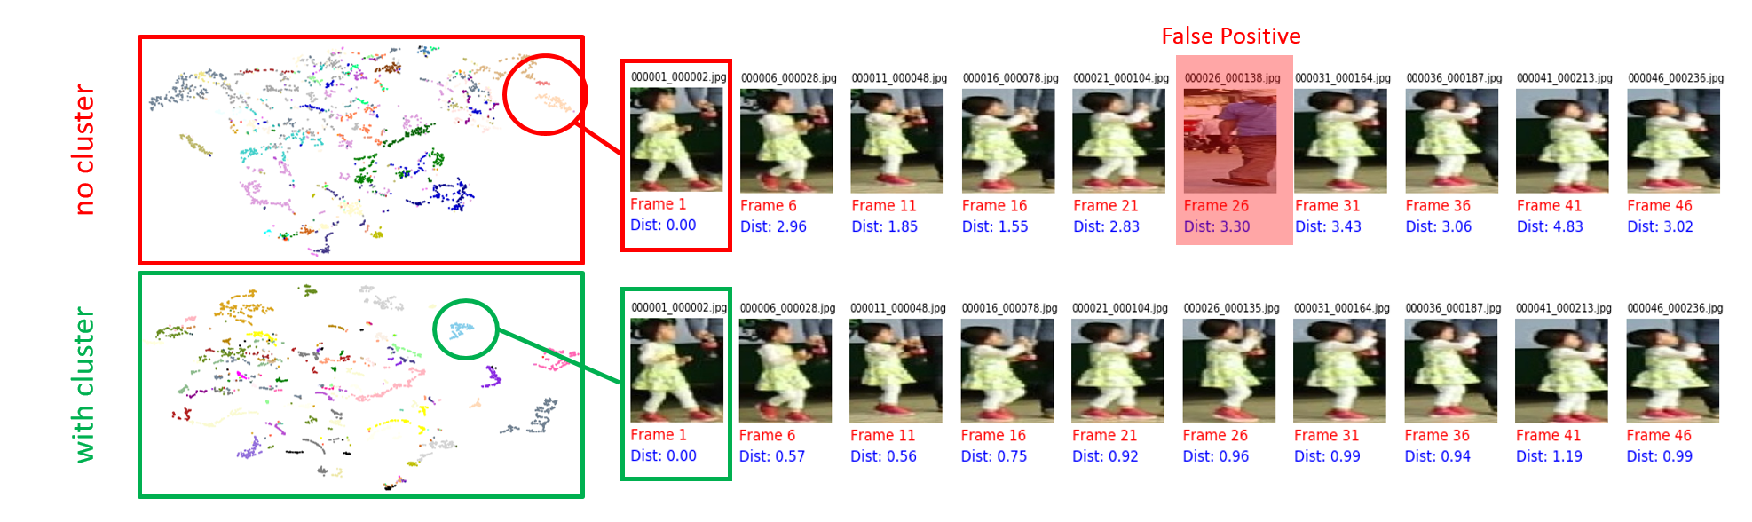
\includegraphics[width=1.0\linewidth]{Fig_4_figure.pdf}
	\end{center}
	\caption{Nearest Neighbor of the query detection (left) within 40 \AK{46 frames} frames with a step size of 5 frames of the sequence MOT17-09-SDP. The second row shows a False Positive neighbor. \AK{this is not clear to me.}}
	\label{fig:figure3}
\end{figure*}

Figure~\ref{fig:figure3} shows the nearest neighbor of a selected frame $t$ (left box marked in red) from the sequence MOT17-09 and frame $t+n$. 
The example illustrates that the location of pair detections are close to one another in the latent space even over a long distance of up to 40 frames, although false positives still appear. 
However, the example also shows that change in appearance affects the AutoEncoder distance, further denoted $d_{\mathrm{AE}}$. 
For instance in the first row, frame 1 and frame 6 are very similar due to the same detection position of the person within the bounding box as well as the direction the woman is looking to (face to camera). 
At frame 41, the woman \AK{isn't that a girl? (in fig. 3)} slightly turned her face to the right. 
Although the correct nearest neighbour was retrieved, the distance $d_{\mathrm{AE}}$ almost doubled.
Another observation is that the position of the bounding box influences the latent space distance.
In the second row, the first detection from the left (frame 5), the detection of the person is slightly shifted to the left. 
At frame 15, 20 or 25, the position is slightly zoomed and $d_{\mathrm{AE}}$ increases \AK{which figure exactly it is referring to?}.

\begin{figure}[!t]
	\begin{center}
		%\fbox{\rule{0pt}{2in} \rule{0.9\linewidth}{0pt}}
		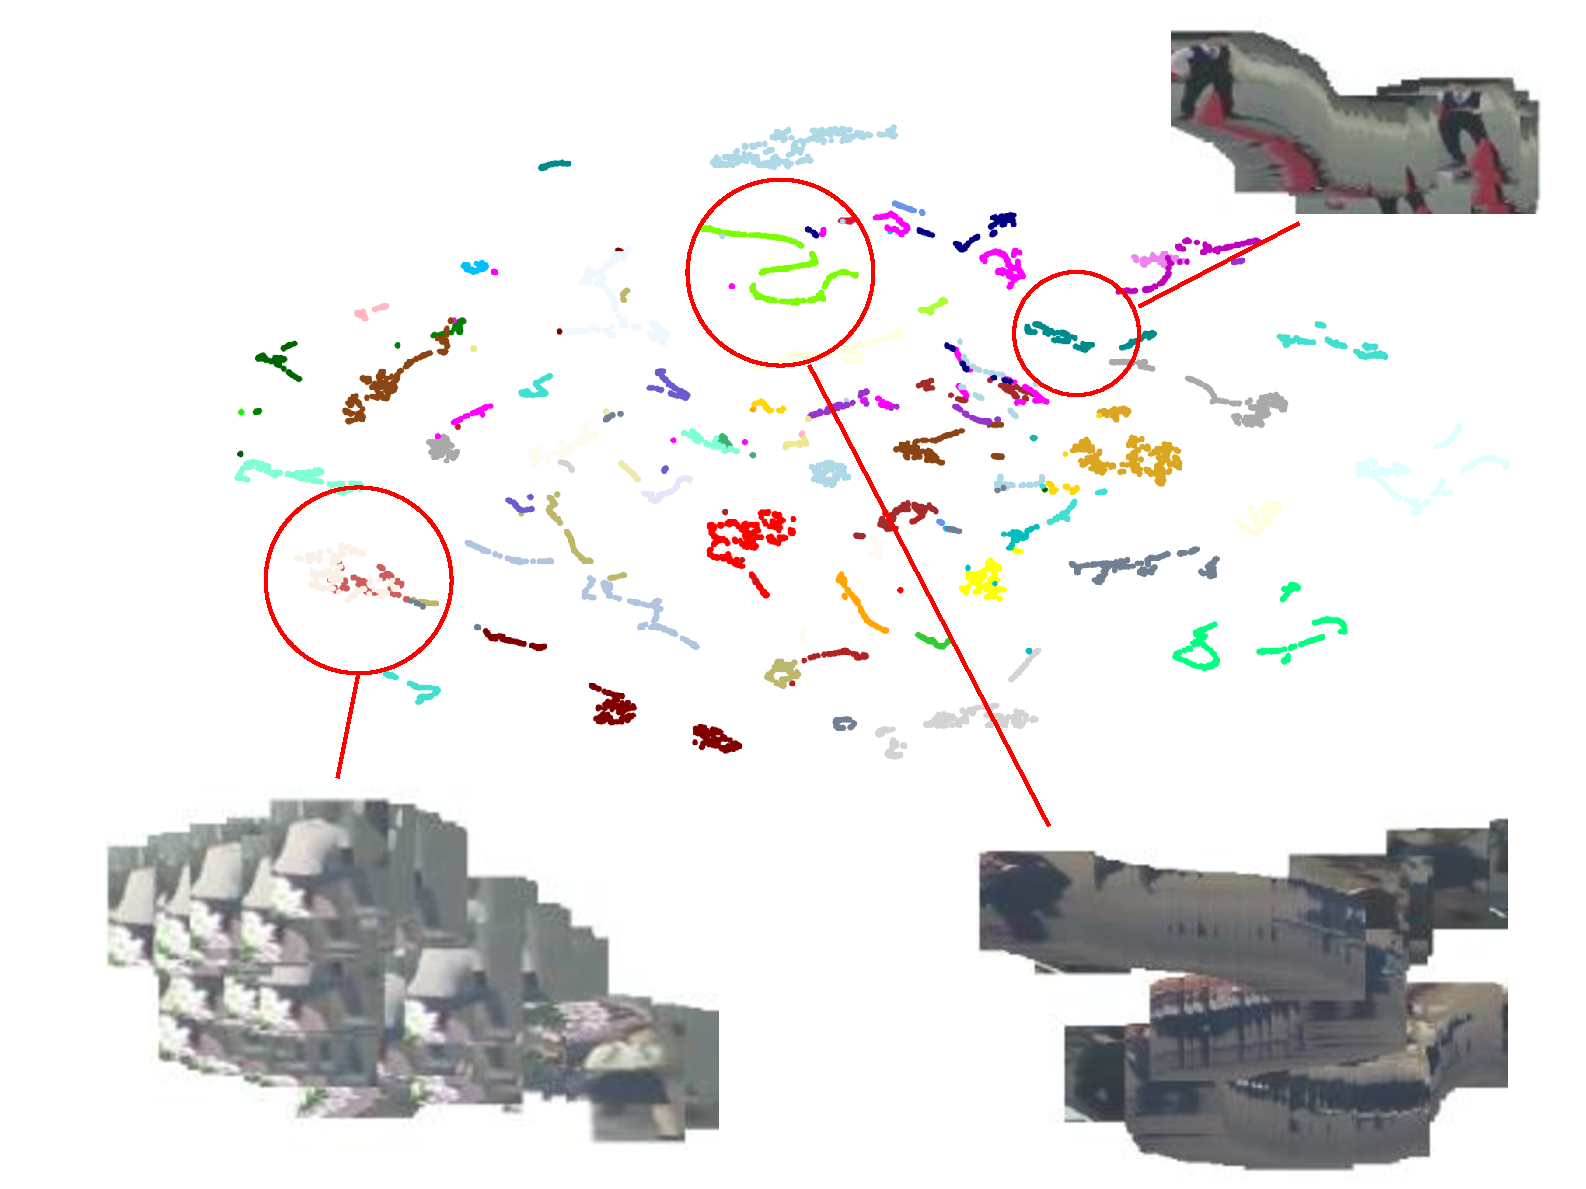
\includegraphics[width=0.9\linewidth]{Fig_5_figure.pdf}
	\end{center}
	\caption{TSNE Visualization of the latent space of the trained auto-encoder for the sequence MOT17-04 FRCNN. The colors represent the assigned person IDs.}
	\label{fig:graph4}
	
\end{figure}

Figure \ref{fig:graph4} shows the TSNE-Visualization \cite{maaten2008visualizing} of the latent space from the sequence MOT17-04-FRCNN. 
Our proposed auto-encoder learned the visual features without supervision. 
The different colors represent the cluster labels. 
As shown in the example circled on the bottom left, similar looking persons are very closed in the latent space: The sitting person in white shirt and the lady, wearing a white shirt (example in bottom left).
The visualization also shows that the same person may change the appearance over time (example on the bottom right). 
In the latent space, the \textit{snake}-like shape may indicate that the viewpoint on a person may have changed over time, causing a continuous appearance change. 
When standing still, the change is minimal, which is also observed in the example on the top right corner.
While for nearby frames, we can compute pairwise cues based on the distance between latent feature representation ($d_{\mathrm{AE}}$), as well as on spatial cues (IoU$_{\mathrm{DM}}$), spatial information can not be used to associate detections over longer temporal distances. 
However, to facilitate the re-identification of objects after being fully or partly occluded, such long-range information is needed.
In these cases, we have to purely rely on the learned latent space distance $d_{\mathrm{AE}}$. 

The distance is directly casted to a binary logistic regression to compute the cut probability of the respective edge in graph $G$. 
The label that is used for the regression comes from the DeepMatching IoU. 
If IoU$_{\mathrm{DM}}(x_i,x_j)<T_{low}$ for a threshold $T_{low}$, $x_i$ and $x_j$ most certainly belong to different objects. 
If IoU$_{\mathrm{DM}}(x_i,x_j)>T_{high}$ for a different threshold $T_{high}$, they are very likely to match. 
Formally, we estimate a probability $p_e \in [0,1]$ between two detections using a feature vector $f^{(e)}$ by regressing the parameters $beta$ \AK{$\beta$?} of a logistic function:

\begin{equation} 
\label{eq:regression} p_e = \frac{1}{1+\exp(-\langle\beta, f^{(e)}\rangle)}
\end{equation} 
Thus, the costs $c_e$ can intuitively be computed by the logit. To robustly estimate these probabilities, we set $T_{low}$ and $T_{high}$ most conservatively to $0.1$ and $0.7$, respectively. 

From this partial, purely spatially induced labeling, we can estimate cut probabilities for all available features combinations, i.e. possible combinations of IoU$_\mathrm{DM}$ and $d_{\mathrm{AE}}$ within nearby frames and only $d_{\mathrm{AE}}$ for distant frames.